\documentclass[8pt]{extarticle}
\usepackage{multicol}
\usepackage{calc}

\usepackage[a4paper,xetex,landscape,left=1cm,right=1cm,
            top=0.7cm,bottom=0.7cm]{geometry}

% Compact titles %%%%%%%%%%%%%%%%%%%%%%%%%%%%%%%%%%%%%%%%%%%%%%%%%%%%%%
\usepackage{titlesec}

\titlespacing*{\section}
{-1.2ex}{0ex}{0ex}
\titlespacing*{\subsection}
{-1.2ex}{0ex}{0ex}
\titlespacing*{\subsubsection}
{-1.2ex}{0ex}{0ex}

\titleformat{\section}
  {\normalfont\sffamily\large\bfseries\color{blue}}
  {\thesection}{1em}{}

\titleformat{\subsection}
  {\normalfont\sffamily\bfseries\color{blue}}
  {\thesubsection}{1em}{}

\titleformat{\subsubsection}
  {\normalfont\sffamily\small\bfseries\color{blue}}
  {\thesubsubsection}{1em}{}
%%%%%%%%%%%%%%%%%%%%%%%%%%%%%%%%%%%%%%%%%%%%%%%%%%%%%%%%%%%%%%%%%%%%%%%

% Don't print section numbers
\setcounter{secnumdepth}{1}

% no space before new paragraph
\setlength{\parindent}{0pt}
\setlength{\parskip}{0pt}

% Turn off header and footer
\pagestyle{empty}
 
\usepackage{tabulary}
% make tabulary prevent overflows (https://tex.stackexchange.com/a/195088)
\tymin=60pt
\tymax=\maxdimen

\usepackage[table,usenames,dvipsnames]{xcolor}
\usepackage[most]{tcolorbox}
\usepackage{fontspec}
\usepackage[urlbordercolor=blue,linkbordercolor=cyan,
            pdfborderstyle={/S/U/W 1}]{hyperref}

% declare font faces for Nunito font https://fonts.google.com/specimen/Nunito
% I don't use package `nunito` since it's not present in older Linux boxes,
% but instead download directly. Also in my installation presence of
% Nunito-VariableFont_wght.ttf/Nunito-Italic-VariableFont_wght.ttf broke
% some font shapes finding so I deleted it leaving only "static" ttf fonts.

\setmainfont{Nunito}[
    FontFace={el}{n}{Font=* ExtraLight},
    FontFace={l}{n}{Font=* Light},
    FontFace={r}{n}{Font=*},
    FontFace={m}{n}{Font=* Medium},
    FontFace={sb}{n}{Font=* SemiBold},
    FontFace={b}{n}{Font=* Bold},
    FontFace={eb}{n}{Font=* ExtraBold},
    FontFace={xb}{n}{Font=* Black},
    FontFace={eli}{i}{Font=* ExtraLight Italic},
    FontFace={i}{i}{Font=* Italic},
    FontFace={mi}{i}{Font=* Medium Italic},
    FontFace={sbi}{i}{Font=* SemiBold Italic},
    FontFace={bi}{i}{Font=* Bold Italic},
    FontFace={ebi}{i}{Font=* ExtraBold Italic},
    FontFace={xbi}{i}{Font=* Black Italic},
]

\DeclareRobustCommand{\elseries}{\fontseries{el}\selectfont}
\DeclareRobustCommand{\lseries}{\fontseries{l}\selectfont}
\DeclareRobustCommand{\rseries}{\fontseries{r}\selectfont}
\DeclareRobustCommand{\mseries}{\fontseries{m}\selectfont}
\DeclareRobustCommand{\sbseries}{\fontseries{sb}\selectfont}
\DeclareRobustCommand{\bseries}{\fontseries{b}\selectfont}
\DeclareRobustCommand{\ebseries}{\fontseries{eb}\selectfont}
\DeclareRobustCommand{\xbseries}{\fontseries{xb}\selectfont}
\DeclareRobustCommand{\eliseries}{\fontseries{eli}\fontshape{i}\selectfont}
\DeclareRobustCommand{\liseries}{\fontseries{li}\fontshape{i}\selectfont}
\DeclareRobustCommand{\iseries}{\fontseries{i}\fontshape{i}\selectfont}
\DeclareRobustCommand{\miseries}{\fontseries{mi}\fontshape{i}\selectfont}
\DeclareRobustCommand{\sbiseries}{\fontseries{sbi}\fontshape{i}\selectfont}
\DeclareRobustCommand{\biseries}{\fontseries{bi}\fontshape{i}\selectfont}
\DeclareRobustCommand{\ebiseries}{\fontseries{ebi}\fontshape{i}\selectfont}
\DeclareRobustCommand{\xbiseries}{\fontseries{xbi}\fontshape{i}\selectfont}

% redefine default bold to extra bold
\DeclareRobustCommand{\bfseries}{\fontseries{eb}\fontshape{n}\selectfont}
% fix \textit
\DeclareTextFontCommand{\textit}{\iseries}

% font for headings
\setsansfont{Open Sans}

% some bolder font
\usepackage{unicode-math}
\setmathfont[Scale=1.0]{TeX Gyre Schola Math}

\usepackage{tikz}
\usetikzlibrary{shapes,arrows,positioning,calc,fit}
\tikzset{
block/.style = {draw, fill=white, rectangle, minimum height=3em, minimum width=3em},
line/.style={-latex},
}

% definition for drawing arrow
\newcommand{\tikzmark}[1]{\tikz[overlay,remember picture] \node (#1) {};}
\newcommand{\DrawBottomReverse}[2]{%
  \begin{tikzpicture}[overlay,remember picture,-latex,shorten >=5pt,shorten
      <=5pt,out=225,in=315]
      \draw[distance=0.45cm,#1] (a.south) to node[right,xshift=1.1cm]{#2}
      (b.south);
  \end{tikzpicture}
}

\newtcolorbox{prebox}[1][]{
    left=0.5mm, right=0.5mm, top=0mm, bottom=0mm,
    before skip=3pt, after skip=3pt,
    frame hidden, boxrule=0.05em,
    colback=green!15, #1}

% colored box around code
\newenvironment{code}[1][]{%
\begin{prebox}[#1]\obeylines%
\fontdimen2\font=0.9ex% inter word space
}{%
\end{prebox}%
\fontdimen2\font=0.6ex% inter word space
}

% box with modifiable size
\newenvironment{codem}[1][\linewidth]{%
\begin{minipage}{#1}%
\begin{prebox}\obeylines}{%
\end{prebox}%
\end{minipage}}

% box with size 90%
\newenvironment{code9}{\begin{codem}[0.9\linewidth]}{\end{codem}}

% inline color box for code
\newcommand{\cod}[1]{\tcbox[
    size=fbox,
    on line,
    colback=green!15,
    colframe=black,
    arc=0.3em  % rounded corners
]{#1}}

% Syntax highlighting for code %%%%%%%%%%%%%%%%%%%%%%%%%%%%%%%%%%%%%%%%
\newcommand{\ind}{\hphantom{~~~}}
% shell and other prompts
\newcommand{\prompt}{\textcolor{red}{\textbf{\$}\ }}
% target prompt:
\newcommand{\tprompt}{\textcolor{brown}{\textbf{target\$}\ }}
\newcommand{\sprompt}{\textcolor{blue}{\textbf{>}\ }}
% Syntax:
\newcommand{\kw}[1]{\textcolor{magenta}{\textbf{#1}}}
\newcommand{\ty}[1]{\textcolor{Orange}{\textbf{#1}}}
% Misc highlighting:
\newcommand{\hl}[1]{\textcolor{blue}{\textbf{#1}}}
% shell/simics script/python comment
\newcommand{\cmtcommon}[1]{\textcolor{Sepia}{\textbf{#1}}}
\newcommand{\cmt}[1]{\cmtcommon{\#\ #1}}
% DML/C comment:
\newcommand{\cmtd}[1]{\cmtcommon{/\,/\ #1}}
\newcommand{\p}[1]{\textit{\large#1}}
%%%%%%%%%%%%%%%%%%%%%%%%%%%%%%%%%%%%%%%%%%%%%%%%%%%%%%%%%%%%%%%%%%%%%%%

\fontdimen2\font=0.6ex% inter word space

\newcommand{\vshort}[1]{%
\vspace{-0.6em}%
#1%
\vspace{-0.3em}}

% This document specific declarations %%%%%%%%%%%%%%%%%%%%%%%%%%%%%%%%%
\newcommand{\local}{\kw{local} }
\usepackage{underscore}  % underscore is often used in code here
\newcommand{\Simics}{\textcolor{cyan}{\textbf{Simics}}}

\newlength{\MyLen}
%%%%%%%%%%%%%%%%%%%%%%%%%%%%%%%%%%%%%%%%%%%%%%%%%%%%%%%%%%%%%%%%%%%%%%%

\begin{document}

% Never allow text overflow to margin:
\setlength\emergencystretch{\hsize}\hbadness=10000


\begin{multicols*}{3}
    %\begin{center} \textbf{\Large \Simics{} Cheat Sheet} \end{center}

\section{\Simics{} Usage}

\subsection{Glossary \& Documentation}
    \settowidth{\MyLen}{\textit{[simics]-script.}}
    \begin{tabular}{p{\the\MyLen}p{\linewidth-\the\MyLen-0.8cm}}
    %\begin{tabular}{@{}p{\the\MyLen}@{}p{\linewidth-\the\MyLen}@{}}
        \textit{\Simics{} Base} & \cod{simics} executable + the set of
        supporting shared libraries (DLLs) + tools
        \\
        \textit{simulation}  & running of code (target) on
        a model/platform (target) with advancement of time
        \\
        \textit{host}        & a computer where simulation runs
        \\
        \textit{target}      & a simulated
        code running in its isolated memory region, e.g. Linux or
        Windows guest
        \\
        \textit{a Platform}  & a complete runnable model:
        full set-up of devices
        with CPU or with at least a clock provider
        \\
        \textit{a Package}   & a set of devices, oftentimes constituting
        1 platform, distributed as a whole in an archive and unpacked
        into 1 directory
        \\
        \textit{[\Simics] Script} & simple Unix-shell-like language (a wrapper
        over Python) used for connecting devices and command line 
        automation
        \\
        \textit{Simics User’s Guide} & documentation on \Simics{}
        usage — both command line and Eclipse
    \end{tabular}

    Below \prompt stands for Unix shell prompt, \sprompt for \Simics{} prompt.

\subsection{Set up a workspace with platform package}
    \begin{code}
        \prompt \p{path/to/simics-base}/bin/project-setup\ \ .
        \prompt bin/addon-manager -c
        \cmt{allow scripts \& shared libraries be found:}
        \prompt bin/addon-manager -s /path/to/platform-package
        \prompt bin/addon-manager -s /path/to/additional/package
    \end{code}

\subsection{Start up}
    \begin{code}
        \prompt ./simics targets/\p{platf/platf.simics}
    \end{code}

    
    %\begin{tabular}{|p{6cm}| p{10cm} |}
    Shell command line arguments $\longrightarrow$ \Simics{} command line 
        correspondence:

    \begin{tabular}{lp{0.9\linewidth}}
        &
        \begin{code9}
            \prompt ./simics start.simics
        \end{code9}
        \vspace{0.05cm}
        \\
        $\longrightarrow$ &
        \begin{code9}
            \prompt ./simics
            \sprompt run-command-file start.simics
        \end{code9}
        \vspace{0.2cm}
        \\

        & \begin{code9}
            \prompt ./simics script.py
        \end{code9}
        \vspace{0.05cm}
        \\
        $\longrightarrow$ &
        \begin{code9}
            \prompt ./simics
            \sprompt run-python-file script.py
        \end{code9}
        \vspace{0.2cm}
        \\

        & \begin{code9}
            \prompt ./simics -e ‘\$config_variable1=value; \$config_var2=value’ start.simics

            \cmt{but NOT ./simics start.simics -e \$varibables ...}
        \end{code9}
        \vspace{0.05cm}
        \\
        $\longrightarrow$ &
        \begin{code9}
            \prompt ./simics
            \sprompt \$config_variable=value
            \sprompt \$config_var2=value
            \sprompt run-command-file start.simics
        \end{code9}
    \end{tabular}


    To debug chain of called auxiliary scripts \cod{include}s:
    \begin{code}
        \prompt ./simics -script-trace targets/\p{platf/platf.simics}
    \end{code}

\subsection{Printing device structure}
To find devices by name/class or interface name:
    \begin{code}
        \sprompt list-objects -all \p{name} \ind \# searches also class
        \sprompt list-objects -all iface = \p{my_interface}
    \end{code}

To find all objects with the same class as given device:
        \begin{code}
            \sprompt \p{platf.myDevice}->classname
            \p{my_class}
            \sprompt list-objects -all class = \p{my_class}
        \end{code}

\subsection{Registers}
\begin{code}
    \cmt{print all registers:}
    \sprompt print-device-regs \p{platf.myDevice}
    \cmt{print fields of register \p{myRegister}:}
    \sprompt print-device-reg-info \p{platf.myDevice.myBank.myRegister}
\end{code}

\subsubsection{Writing/reading with side effects}

\begin{code}
    \sprompt write-device-reg
    \ind \ind \p{platf.myDev}.bank.\p{myBank.myGrp.myReg} 0x1
    \cmt{(Register group \p{myGrp} may be absent in devices)}
    \sprompt read-device-reg \p{platf.myDev}.bank.\p{myBank.myGrp.myReg}
\end{code}

%\subsubsection{Writing/reading \textbf{without} side effects (aka set/get)}
\subsubsection{Writing/reading {\bseries without} side effects (aka set/get)}

It's done through attributes:
\begin{code}
    \cmt{To set to value 0x1}
    \p{platf.myDev}->\p{myBank_myGrp_myReg} = 0x1
    \cmt{To get the value:}
    \p{platf.myDev}->\p{myBank_myGrp_myReg}
\end{code}


\subsection{Running commands}
\begin{code}
\sprompt c[ontinue]
\sprompt r[un] 100 cycles \ind \# or 10 steps or 0.1 seconds
\sprompt ptime [-all] \ind \# to show target's time
\end{code}

\subsection{Debugger commands}
To use \Simics{} to debug target:
\begin{code}
dis[assemble] — show assembler commands at current address

\# Break points
break address
break-hap Core-Magic-Instruction
\end{code}

\subsection{Examining current state}

\begin{tabular}{ll}
    pselect & show currently running CPU \\
    memory-map & print all mapped devices \\
    pregs & print all CPU registers \\
    probe-address \p{addr} & path to target \p{addr}
\end{tabular}

\subsection{x86-specific and platform-specific commands}

\begin{tabular}{ll}
    memory-trace \p{addr} & path to target \p{addr} \\
    pregs & to know x86 mode (16/32/64-bit), 1st line \\
    reset-button-press & to reboot the target \\
    power-button-press & to press power button \\
\end{tabular}

\subsection{Moving files target \texorpdfstring{$\longleftrightarrow$}{<->} host}
%\subsection{Moving files target $\longleftrightarrow$ host}
%\subsection{Moving files target <-> host}
\begin{code}
\sprompt start-simicsfs-server
\end{code}

\begin{code}[colback=blue!15]
\tprompt mkdir a
\tprompt simicsfs-client a
\end{code}

\subsection{Saving info}
Save logs from current point
\begin{code}
\sprompt start-command-line-capture
\end{code}

Save simics variables to file
\begin{code}
\sprompt start-command-line-capture
\sprompt list-variables
\sprompt stop-command-line-capture
\end{code}

\subsection{Check points}
\begin{tabular}{ll}
            \cod{write-configuration \p{"checkpoint_name"}} & — save
            checkpoint \\
            \cod{read-configuration \p{"checkpoint_name"}} & — restore it back
\end{tabular}

\subsection{Model information}

\begin{code}
    \cmt{Documentation + information about class\&module:}
    \sprompt help \p{platf.myDev}
    \cmt{pretty-print device attributes with values:}
    \sprompt list-attributes \p{platf.myDev}
    \cmt{Configuration information}
    \sprompt \p{platf.myDev}.info
    \cmt{Runtime information:}
    \sprompt \p{platf.myDev}.status
\end{code}

\subsection{Environment}
\begin{code}
    \sprompt version  \cmt{list of installed packages}
    \prompt ./simics -v \cmt{the same}
    \sprompt pwd \cmt{current directory where simics is running}
\end{code}

\subsection{Making images}

\newpage

\section{\Simics{} DML 1.4 Programming \& C/DML API}

\subsection{Glossary \& Documentation}
    \settowidth{\MyLen}{\texttt{dml-1.4-reference-man}}
    %\begin{tabulary}{\linewidth}{p{4cm}L}
    \begin{tabular}{p{\the\MyLen}p{\linewidth-\the\MyLen-0.8cm}}
        \textit{DML}         & Device Modelling Language (its compiler 
        is included into \Simics{} Base) used for writing (fast) devices
        \\
        \kw{device}          & any \Simics{} class for modelling real
        devices. Different \Simics{} devices communicate via interfaces
        \\
        \textit{Model Builder User’s Guide} & overview of Simics/DML
        programming \\
        \textit{DML 1.4 Reference Manual} & language specification \\
        \textit{API Reference Manual} & API function list for DML \& C,
        describes ownership rules
    \end{tabular}

\subsection{Create stub device}

\begin{code}
    \prompt bin/project-setup -{}-device \p{example-dev}
    \prompt ls modules/\p{example-dev}
    test/  \p{example-dev}.dml  Makefile  module_load.py
\end{code}

The header of \p{example-dev}.dml is then:

\begin{code}
    %\begin{tabulary}{\linewidth}{p{4cm}L}
    %\begin{tabular}{p{3cm}p{\linewidth-3.8cm}}
    \begin{tabular}{ll}
        dml 1.4;                  & \cmtd{Obligatory .dml header} \\
        \kw{device} example_dev;  & \cmtd{Class name.} \\
                                  & \cmtd{Note: - changed to underscore _}
    \end{tabular}
\end{code}

\subsection{Create stub interface with Python wrapper}

\begin{code}
    \prompt bin/project-setup -{}-interface \p{sample}
    \prompt ls modules/\p{sample}-interface
    Makefile  \p{sample}-interface.dml  \p{sample}-interface.h
\end{code}

Python support is enabled by \cod{IFACE_FILES} in the Makefile.
The generated C \kw{struct} name is \cod{\p{sample}_interface_t}.

\subsection{Arithmetics}

\subsubsection{RHS is int64, LHS truncates}

Assignments are equivalent to casts and hence can truncate:
        \begin{code}
            \local \ty{uint8} x = 0xffff  \cmtd{results in x == 0xff}
        \end{code}

        All aritmetic operators like $+$, $*$ convert its operands to int64:
        \begin{code}
            \local \ty{uint16} $i$ = 0x7fff; \local \ty{int8} $j$ = 2;  \cmtd{let us sum them:}
            \vspace{0.1cm}
            \local \ty{int16} \tikzmark{b} $x$ = $\overbrace{\ind i + j; \ind }^{\text{calculates as int64 $\rightarrow$ 0x8001} \tikzmark{a}}$ \DrawBottomReverse{black}{truncates to int16} \cmtd{finally results in $x == 1$}
            \vspace{0.3cm}
        \end{code}


\subsubsection{Comparisons act as uint64 or int64: $==$, $<$, $<=$}
Comparisons on only uint64 act as proper uint64, however
in comparisons int64 vs. uint64 the operands are converted to int64!

        \begin{code}
            \local \ty{uint64} u;
            u = -1; \ind \cmtd{equivalent to u = cast(-1, uint64) $\mathbf{= 2^{64}-1}$, all ones}
            \begin{tabular}{@{}ll}
                u == -1 & \cmtd{FALSE! Equivalent to int64(u) == int64(-1),} \\
                        & \cmtd{where upper bit is cropped: int64(u) == ($\mathbf{2^{63}-1}$).}
            \end{tabular}
            u == cast(-1, \ty{uint64}) \cmtd{true. As comparison is b/w two uint64}
            u > -1 \ind \cmtd{true, but unlike C! it's int64(u) > int64(-1): $\mathbf{2^{63}-1>1}$}
        \end{code}

\subsection{Syntax}

    \subsubsection{Statements}

    \subsubsection{Types}

    \subsubsection{Methods}

\subsubsection{Module variables and other data objects}

\rowcolors{2}{gray!15}{white}
    \global\rownum=1\relax
    \begin{tabulary}{\linewidth}{|LLLLL|}
        \hline
        DML construct & checkpointed & fields & address-mapped & arbitrary data\\
        \hline
        \kw{session} & - & - & - & + \\
        \kw{saved} & + & - & - & - \\
        attribute & + & - & - & + \\
        unmapped register & + & + & - & - \\
        {[}normal{]} register & + & + & + & - \\
        \hline
    \end{tabulary}

    \subsubsection{Interfaces}

    Definition in \cod{.dml}:
    \begin{code}
        extern typedef \kw{struct} \{
            \ind method \p{name}(\p{\ty{$type_1$} $value_1$}) -> \p{\ty{out_type}};
        \} \ty{\p{sample}_interface_t};
    \end{code}

    Obligatory definition in C \cod{.h} file:
    \begin{code}
        SIM_INTERFACE(\p{sample}) \{  \cmtd{essentially 'typedef \kw{struct}' also}
            \ind \ty{\p{out_type}} (*\p{name})(\ty{conf_object_t *} \hl{obj}, \ty{\p{$type_1$}} \p{$value_1$});
        \}
    \end{code}

    \subsubsection{Explaining \cod{connect}s and \cod{implement}s}

    \begin{itemize}
        \item \cod{connect}s are for \textbf{out}bound calls
        \item \cod{implement}s are for \textbf{in}bound calls
    \end{itemize}

    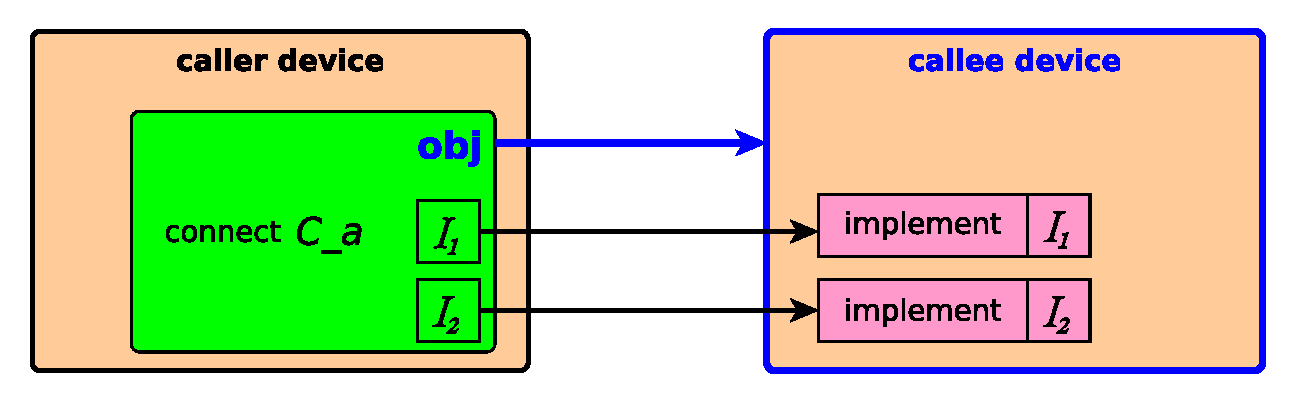
\includegraphics[width=\linewidth]{diagrams/connect_implement.pdf}

    \global\rownum=1\relax
    %\begin{tabulary}{\linewidth}{|lcc|}
    \begin{tabular}{|lp{2.5cm}c|}
        \hline
        %co & \begin{minipage}{2.5cm}unnamed (whole-device)\end{minipage} & 
         & unnamed (whole-device) & named \\
        \hline
        \cod{connect} & - &
            \begin{codem}[3cm]
                connect \p{C_a} \{
                  \ind interface $I_1$ \{
                      \vshort{\ind\ind ...}
                  \ind \}
                  \ind interface $I_2$ \{
                      \vshort{\ind\ind ...}
                  \ind \}
                \}
                connect $C_B$ \{
                  \ind interface $I_2$ \{
                    \vshort{\ind\ind ...}
                    %  \vspace{-0.6em}
                    %\ind\ind ...
            \end{codem}
            \\[1.4cm]  % selected by trial
        \cod{implement} &
            \begin{codem}[2.5cm]
                implement $I_1$ \{
                    \ind ...
                \}
                implement $I_2$ \{
                    \ind ...
                \}
            \end{codem}
            (as in picture above)
            &
            \begin{codem}[3cm] 
                port $P_A$ \{
                \ind implement $I_1$ \{
                    \vshort{\ind\ind ...}
                \ind\}
                \ind implement $I_2$ \{
                    \ind\ind \emph{... variant 1 ...}
                      \vspace{-0.3em}
                \ind\}
                \}
                port $P_B$ \{
                \ind implement $I_2$ \{
                    \ind\ind \emph{... variant 2 ...}
            \end{codem}
            \\
        \hline
    \end{tabular}

    To make interface required:
        \begin{code}
            \kw{param} required = true;
        \end{code}
    To make the whole \cod{connect} required:
        \begin{code}
            \kw{param} configuration = "required";
            \# other options: "optional", "pseudo", TODO
        \end{code}

\subsection{Debugging with Gdb}
To debug simics and its modules itself:
        \begin{code}
            \cmt{Terminal \#1:}
            \prompt make clobber-\p{my-module}
            \prompt make D=1 \p{my-module}
            \prompt ./simics
            \sprompt pid
            \p{12345}
        \end{code}

        \begin{code}[colback=blue!15]
            \cmt{Terminal \#2:}
            \prompt bin/gdb
            >\,>\,> attach \p{12345}
            >\,>\,> br \p{file.dml:100}  \ind \# break on line 100
            >\,>\,> continue
        \end{code}

        \begin{code}
            \cmt{Back to terminal \#1:}
            \sprompt run-command-file targets/\p{platf/platf.simics}
        \end{code}


\subsubsection{Using gdb for debugging target}
\begin{code}
    load-module gdb-remote
    new-gdb-remote \p{50000}  \ind \# open port \p{50000}
\end{code}


\subsection{Attribute values}
    \cod{attr_value_t} is a C union that can hold one of a
    few predefined types.

    Attributes values are allocated/packed by:\\
    \cod{attr_value_t x = \textbf{SIM_make_attr_\p{T}}(\p{cType} val)},
    and extracted by:\\
    \cod{\p{cType} \ind \ind val = \textbf{SIM_attr_\p{T}}(x)}, where
    \p{T} and \p{cType} can be:

        \global\rownum=0\relax
        \begin{tabulary}{\linewidth}{|LLL|}
            \hline
            \p{T}         & type spec & \p{cType} — DML/C type \\
            \hline
            uint64, int64 & i & \ty{uint64}, \ty{int64} \\
            boolean       & b & \ty{bool} \\
            floating      & f & \ty{double} \\
            string        & s & \ty{char*} \\
            object        & o & \ty{conf_object_t} \\
            list          & [\ty{$x_1$}...\ty{$x_n$}] & fixed-width tuple with $n$ elements of types \ty{$x_1$}, ..., \ty{$x_n$} \\
            list          & [\ty{$x$}*] & arbitrary-width array of \ty{$x$} \\
            list          & [$x+$] & non-empty arbitrary-width array
                                     of \ty{$x$} \\
            list          & [\ty{$x$}$\{m:n\}$] & array of \ty{$x$} with $m ≤ size ≤ n$ \\
            list          & [\ty{$x$}$\{n\}$] & fixed-width tuple with $n$
                                         elements of \ty{$x$} \\
            dict          & D & array of \ty{attr_dict_pair_t} \\
            data          & d & \ty{uint8*} \\
            nil           & n & \ty{void} or \ty{$x$*} \\
            invalid       &   &  (none, used for indicating errors) \\
            \hline
        \end{tabulary}

    List items are accessed by \cod{SIM_attr_list_item}.
    Type specs can be OR'ed as \cod{$x_1$\kw{|}$x_2$}.
    Type spec is used in \cod{\kw{param} type = "..."}. For first 4
    types there are predefined DML templates \cod{uint64_attr},
    \cod{int64_attr}, \cod{bool_attr}, \cod{double_attr}.

    \renewcommand\_{\textunderscore\linebreak[1]}

\subsection{Attribute initialization}
    %\begin{tabulary}{\linewidth}{|LLL|}
        \global\rownum=0\relax
        \begin{tabulary}{\linewidth}{|p{3.5cm}p{2cm}p{2.2cm}|}
        \hline
        Execution stage & SIM_object_is_configured(obj) &
            SIM_is_restoring_state(\,) \\
        \hline
        Create object at 1st platform init & - & - \\
        Load checkpoint & - & + \\
        Load micro-checkpoint (reverse execution) & + & + \\
        Manual attribute assignment (hot plug from \Simics{} command line) & + & - \\
        \hline
    \end{tabulary}

\subsection{Standard register templates}

\subsection{Compile-time statements \& conditional compilation}

\subsection{Hash tables}

        \begin{code}
            \kw{import} "simics/util/hashtab.dml";
            \vshort{...}
            \local \ty{ht_str_table_t} tab;  \cmtd{str — string (aka const char*) keys.}
            ht_init_str_table(\kw{\&}tab, \cmtcommon{/*keys_owned*/} true);
            \local \ty{double *}value = new \ty{double};  \kw{*}value = 10.0;
            ht_insert_str(\kw{\&}table, "key", cast(value, \ty{void *}));
            \local \ty{double *}get_back = cast(ht_lookup_str(\kw{\&}tab, "key"), \ty{double*});
            assert \kw{*}get_back == 10.0;
        \end{code}
        There are also tables for \cod{\ty{int}} keys or general (\cod{common}) keys.

\subsection{The secret of DML}
        Many "internal" features like registers and even connects are actually
        normal templates for objects (\cod{\kw{is} object;}) in plain DML
        defined in \texttt{1.4/dml-builtins.dml} and thus they can be expanded.

\subsection{C API}

It's possible to do most things in C, e.g. create device by
\cod{SIM_create_object}, though normally it's done from Python components.

\newpage


\section{\Simics{} configuration and build system}

\subsection{Glossary \& Documentation}
    \settowidth{\MyLen}{\texttt{Components}}
    %\begin{tabulary}{\linewidth}{p{4cm}L}
    \begin{tabular}{p{\the\MyLen}p{\linewidth-\the\MyLen-0.8cm}}
        \textit{Python}      & this language is used for connecting 
        devices together (writing components), for writing
        some (slow) devices, for unit-testing
        \\
        \textit{Component}  & a special \Simics{} class that implement:
        required: \cod{component} interface
        optional: \cod{component_connector} interface

    \end{tabular}

\subsection{Creating devices dynamically}
\begin{code}
\sprompt create-myDevice-comp
\sprompt connect $system.mydev$ system.some.connect
\sprompt instantiate-components
\end{code}

\subsection{Modules/Components/Classes}
A \Simics{} module includes classes, there are 2 types of them:
        \begin{itemize}
            \item devices, typically written in DML
            \item \textit{components}, typically written in Python
        \end{itemize}
%In simplest case there are no components:
%
%\begin{tikzpicture}
%
%    \node[block, fill=lightgray] (a) {\p{block_a} (DML device)};
%    \node[above of=a] (am) {block-a module};
%    \node[draw, fill=gray, fill opacity=0.5, inner xsep=3mm,
%          inner ysep=1mm, fit=(a)(am)] (m) {};
%
%\end{tikzpicture}


A typical layout with 1-to-1 device-component correspondence:

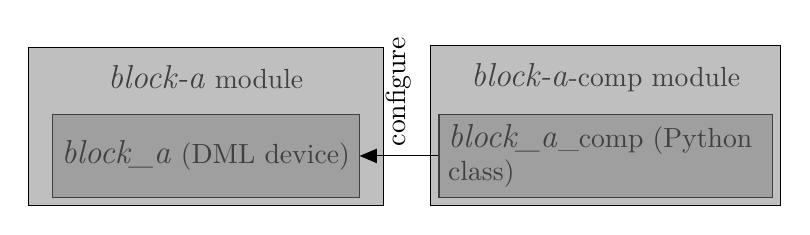
\begin{tikzpicture}
    \node[block, fill=lightgray] (a) {\p{block_a} (DML device)};
    \node[above of=a] (caption) {\p{block-a} module};
    \node[draw, fill=gray, fill opacity=0.5, inner xsep=3mm,
          inner ysep=1mm, fit=(a)(caption)] (am) {};
    
    \node[block, right=1cm of a, fill=lightgray, text width=4cm] (ac) 
        {\p{block_a}_comp (Python class)};
    \node[above of=ac] (acm) {\p{block-a}-comp module};
    \node[draw, fill=gray, fill opacity=0.5, inner xsep=1mm,
          inner ysep=1mm, fit=(ac)(acm)] (cm) {};
    
    \draw[-triangle 45] (ac)-- (a) node[midway,right,rotate=90]{configure};
\end{tikzpicture}

In simplest case there are no components for a device, so its
platform \p{platf} will have to instantiate and configure the device:

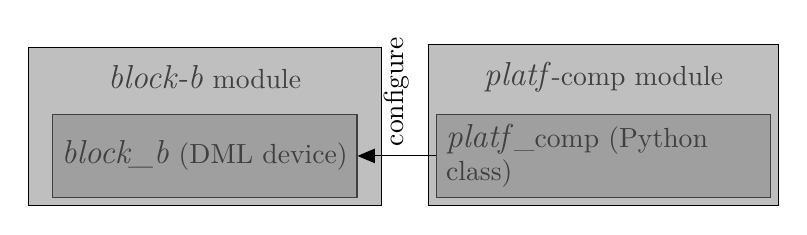
\begin{tikzpicture}
    \node[block, fill=lightgray] (b) {\p{block_b} (DML device)};
    \node[above of=b] (bm) {\p{block-b} module};
    \node[draw, fill=gray, fill opacity=0.5, inner xsep=3mm,
          inner ysep=1mm, fit=(b)(bm)] (am) {};
    
    \node[block, right=1cm of b, fill=lightgray, text width=4cm] (pc) 
        {\p{platf}_comp (Python class)};
    \node[above of=pc] (pcm) {\p{platf}-comp module};
    \node[draw, fill=gray, fill opacity=0.5, inner xsep=1mm,
          inner ysep=1mm, fit=(pc)(pcm)] (cm) {};
    
    \draw[-triangle 45] (pc)-- (b) node[midway,right,rotate=90]{configure};
\end{tikzpicture}

There can be a module with 1 component and many classes:

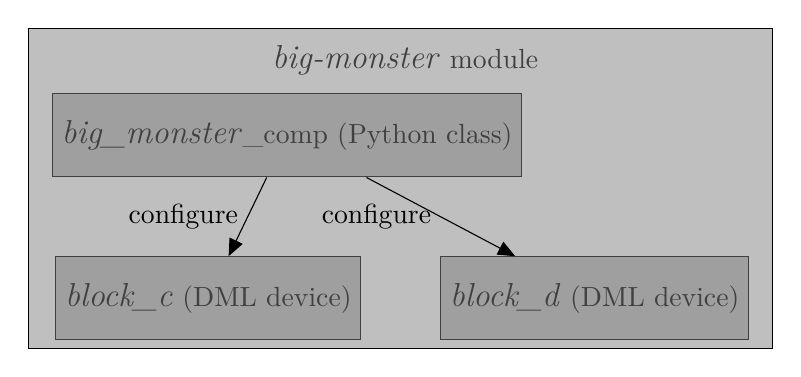
\begin{tikzpicture}
    \node[block, fill=lightgray] (x) {\p{big_monster}_comp (Python class)};
    \node[block, below=of x, fill=lightgray,xshift=-1cm] (c)
        {\p{block_c} (DML device)};
    \node[block, right=of c, fill=lightgray] (d) {\p{block_d} (DML device)};

    \node[xshift=1.5cm, above=0.1cm of x] (caption) {\p{big-monster} module};
    \node[draw, fill=gray, fill opacity=0.5,inner xsep=3mm,inner ysep=1mm, 
    fit=(c)(d)(x)(caption)] {};
    \draw[-triangle 45] (x)-- (c) node[midway,left]{configure};
    \draw[-triangle 45] (x)-- (d) node[midway,left]{configure};
\end{tikzpicture}

\subsection{Connecting devices}
  \begin{itemize}
      \item from Script:
          \begin{code}
              platf.$device_1$->$connect_1$ = platf.$device_2$
          \end{code}
      \item from Python:
          \begin{code}
              conf.platf.$device_1$.$connect_1$ = conf.platf.$device_2$
          \end{code}
  \end{itemize}

\subsection{Structure of components}

\subsection{Calling device code from Python}

Then the interface can be invoked from \Simics{} command line via Python:
\begin{code}
    @conf.platf.device.ifaces.$iface_1$.$method_1$(1, None)
\end{code}

Copyright \copyright\ 2021—2022 Andrey Makarov \\
\href{https://github.com/a-mr/simics-cheatsheet}{https://github.com/a-mr/simics-cheatsheet}
Version 6.0.100

\end{multicols*}
\end{document}
